\documentclass[12pt]{report}
\usepackage[utf8]{inputenc}
\usepackage[T1]{fontenc}
\usepackage[fleqn]{amsmath}
\usepackage{amsfonts,amssymb,stmaryrd}
\usepackage[english]{babel}
\usepackage{pdfpages}

%=============Affichage=======================
\usepackage{fullpage}
\usepackage{mathtools}
\usepackage{lmodern}
\usepackage{xcolor}
\usepackage{enumitem}
\usepackage{tikz,tkz-tab}
\usepackage[ruled,vlined]{algorithm2e}
\usepackage{booktabs}
\usepackage{setspace}
\usepackage{tikz}
\usetikzlibrary{arrows,automata}
\title{TD Statistiques 3A STI}
\author{Waxin Alban}

\definecolor{almond}{rgb}{0.94, 0.87, 0.8}
\definecolor{champagne}{rgb}{0.97, 0.91, 0.81}
\definecolor{dgreen}{rgb}{0.0, 0.5, 0.0}
\definecolor{bc}{rgb}{0.8588, 0.8980, 0.9450}

\setlength{\topmargin}{-1.5cm}
\setlength{\textheight}{25cm}
\setlength{\textwidth}{16cm}
\setlength{\oddsidemargin}{-1.5cm}
\setlength{\evensidemargin}{50cm}
\doublespacing  

\newcommand{\rd}[1]{\textcolor{red}{#1}}
\newcommand{\g}[1]{\textcolor{lime}{#1}}
\newcommand{\dg}[1]{\textcolor{dgreen}{#1}}
\newcommand{\blue}[1]{\textcolor{blue}{#1}}
\newcommand{\cy}[1]{\textcolor{cyan}{#1}}
\newcommand{\blz}{$\blacklozenge$}
\newcommand{\ns}{\\\indent\indent\vspace{0.25cm}}
\setcounter{secnumdepth}{5}% profondeur de la table des matières
\usepackage{titlesec}


\titleformat{\chapter}[frame]
{\Huge}
{\filright\rmfamily\bfseries\Huge\enspace\thechapter\enspace}
{18pt}
{\rmfamily\huge\bfseries\filcenter}
% rmfamily=roman, sffamily = sans serif ou ttfamily =type writer
\usepackage[many]{tcolorbox} % Creation de box collorable pour le texte non intégré
\newtcolorbox{mybox}{colback=bc,
colframe=black,arc=0mm,sharp corners= northwest,arc=10pt}

\newtcolorbox{demo}{colback=almond,
colframe=black,arc=0mm,sharp corners= northeast,arc=10pt}

\renewcommand*{\overrightarrow}[1]{\vbox{\halign{##\cr
 \tiny\rightarrowfill\cr\noalign{\nointerlineskip\vskip1pt}
 $#1\mskip2mu$\cr}}}

\newcommand{\rem}[1]
{
\subparagraph*{\underline{Remarque:#1}}\mbox{}\\
}

\newcommand{\props}[1]
{
\begin{mybox}
\textbf{\rd{\underline{\blz Propriété:} #1}}
\vspace{0.5cm}
\newline
}

\newcommand{\prope}
{
\end{mybox}
}

\newcommand{\scal}[2]
{
<#1|#2>
}

\newcommand{\defis}[1]
{
\begin{mybox}
\textbf{\rd{\underline{\blz Définition:} #1}}
\vspace{0.5cm}
\newline
}
\newcommand{\defie}
{
\end{mybox}
}
\newcommand{\demos}[1]
{
\begin{demo}
\textbf{\underline{\blz Démonstration:} #1}
\newline
}
\newcommand{\demoe}
{
\end{demo}
}
\newcommand{\exe}[1]
{
\subparagraph*{\underline{Exemple:#1}}\mbox{}\\
}

\newcommand{\vs}
{
\vspace{0.25cm}
}

\newcommand{\thms}[1]
{
\begin{mybox}
\textbf{\rd{\underline{\blz Théorème:} #1}}
\vspace{0.5cm}
\newline
}

\newcommand{\thme}
{
\end{mybox}
}

\newcommand{\coros}[1]
{
\begin{mybox}
\textbf{\rd{\underline{\blz Corolaire:} #1}}
\vspace{0.5cm}
\newline
}

\newcommand{\coroe}
{
\end{mybox}
}

\newcommand{\lems}[1]
{
\begin{mybox}
\textbf{\rd{\underline{\blz Lemme:} #1}}
\vspace{0.5cm}
\newline
}

\newcommand{\leme}
{
\end{mybox}
}
%=============================================

%\usepackage[cm]{aeguill}

%=============Mathématiques=================

%--------------Raccourcis:------------------
\newcommand{\R}{\mathbb{R}}
\newcommand{\C}{\mathbb{C}}
\newcommand{\N}{\mathbb{N}}
\newcommand{\Q}{\mathbb{Q}}
\newcommand{\Z}{\mathbb{Z}}
\newcommand{\K}{\mathbb{K}}
\newcommand{\M}{\mathcal{M}}
\newcommand{\nint}[1]{#1 \in \N}
\newcommand{\zint}[1]{#1 \in \N^*}
\newcommand{\limi}[1]{\underset{#1 \to \infty}{lim}}
\newcommand{\limn}[2]{\underset{#1 \to #2}{lim}}
\newcommand{\x}{\times}
\newcommand{\un}[1]{u_{#1}}
\newcommand{\uns}{(u_n)_\nint{n}}
\newcommand{\Sn}[1]{S_{#1}}
\newcommand{\Sns}{(S_n)_\nint{n}}
\newcommand{\ol}[1]{\overline{#1}}
\newcommand{\znz}{\Z/n\Z}
\renewcommand{\o}{\circ}

\newcommand{\seriegu}{\sum u_n}
\newcommand{\seriegv}{\sum v_n}
\newcommand{\harmonique}{\sum \frac{1}{n}}
\newcommand{\SRieman}{\sum \frac{1}{n^\alpha}}
\newcommand{\serie}[3]{\sum_{#1}^{#2}{#3}}
\newcommand{\satps}{série à terme positif}
\newcommand{\satp}{séries à termes positifs}
\newcommand{\pl}[1]{\mathbb{#1}[X]}
\newcommand{\som}[2]{\sum\limits_{#1}^{#2}}


\newcommand{\abs}[1]{\left\lvert#1\right\rvert}
\DeclarePairedDelimiter{\ceil}{\lceil}{\rceil}

%Format de fonctions:
\newcommand{\fct}[5]
	{
	  \begin{array}{ccccc}
		#1 & : & #2 & \to & #3 \\
	    && #4 & \mapsto & #5 \\
	  \end{array}
	}
\newcommand{\dfct}[2] {#1 \mapsto #2}

\renewcommand{\abs}[1]{|#1|}
\newcommand{\nm}[2]{ ||#1||_{#2} }
%===================TESTS===================

\begin{document}
\chapter{Langages Formels}
\section{Exercice 1}
\begin{enumerate}
    \item \begin{align*}
        (KL)^* &= \bigcup_{i=0}^n (KL)^i\\
               &= \lbrace \varepsilon \rbrace \cup (\bigcup_{i=1}^n (KL)^i)\\
               &= \lbrace \varepsilon \rbrace \cup (\bigcup_{i=0}^n(KL)(KL)^{i+1})\\
               &= \lbrace \varepsilon \rbrace \cup (KL)(\bigcup_{n\in \N}(KL)^{n})\\
               &= \lbrace \varepsilon \rbrace \cup (KL)(KL)^*
    \end{align*}
    \demos{LEMME 1: $K(LK)^*L = (KL)(KL)^*$}
        Par démonstration du Lemme 2 suivant, vrais pour tout N donc vrais pour l'union
    \demoe{}
    \demos{LEMME 2 :$K(LK)^nL = (KL)(KL)^n$}
        n=0,  KL = KL\\
        Soit $n \in \N$
        \begin{align*}
            (KL)(KL)^n &=  (KL)(KL)(KL)^{n-1}\\
            HR         &=  (KL)K(LK)^{n-1}L\\
            Associativité  &=  K(LK)(LK)^{n-1}L\\
                       &= K(LK)^n L\\
        \end{align*}
    \demoe{}
    \item Soit $n \in \N^*$ \\
    \begin{align*}
        K^*=\bigcup_{k\in\N}K^k &=\bigcup_{q=0}^{n-1} \bigcup_{m \in [q]}K^m\\
        &= \bigcup_{q=0}^{n-1} \bigcup_{p \in \N}K^{np+q}\\
        &= \bigcup_{q=0}^{n-1} (\bigcup_{p \in \N}K^{np})K^q\\
        &= \bigcup_{q=0}^{n-1} (K^n)^*K^q\\
        &= (K^n)^* \bigcup_{q=0}^{n-1} K^q\\
    \end{align*}
    \item $(K\cup L)^* = \bigcup_{n\in N} (K \cup L)^n$\\
    $\# w = n, \exists u,v \in (K \cup L)^* et l \in L$ tel que $ w = ulv$\\
    or $\# = n $ d'ou $\#u \leq n$ et $\#v \leq n$\\
    Hypothèse: $u,v \in (K^*L)^*K^*$\\
    $w = ulv \in (K^*L)^*(K^*L)(K^*L)^*K^*$\\
    A FINIR
\end{enumerate}
\section{Exercice 2}

$\Sigma = \lbrace 0,1 \rbrace$\\

$n = 2, f_2 = f_1f_0 = 0$; 2 est pair\\
$n = 3, f_3 = f_2f_1 = f_1f_0f_1 = 010$ 3 est impair\\
$n = 4, f_4 = f_3f_1 = 01001$\\

$w_n = \begin{cases}
    01 \text{ si } n\in 2\N\\
    10 \text{ sinon}
\end{cases}$

Montrons qu'il existe $g_n$ tel que $f_n = g_nw_n$\\
$f_n = f_{n-1}f_{n-2} = f_{n-1}g_{n-2}w_{n-2} = f_{n-1}g_{n-2}w_n$\\
$g_n = f_{n-1}g_{n-2} = g_{n-1}w_{n-1}g_{n-2} = (g_{n-2}w_{n-2}g_{n-3})w_{n-1}g_{n-2}$\\
\section{Exercice 3}
\begin{itemize}
    \item \begin{align*}
        \begin{cases}
            A = ( 01^* + 1) A +B\\
            B = 11 + 1A +00C\\
            C = \varepsilon + A +B
        \end{cases} &\Leftrightarrow 
        \begin{cases}
            A = ( 01^* + 1)^*B = \Sigma^* B\\
            B = 11 + 1\Sigma^* B +00 + 00\Sigma^* B + 00B\\
            C = \varepsilon + (00+1)\Sigma^* B = ((00+1)\Sigma^*)^* (00+11) = ((00+1)\Sigma^*)^*(00+11)
        \end{cases}\\
        & \Leftrightarrow
        \begin{cases}
            A = ( 01^* + 1)^*B = \Sigma^* B\\
            B = 11 + 1\Sigma^* B +00 + 00\Sigma^* B + 00B\\
            C = \varepsilon + \Sigma^* (00 + 11) + (00+11) = \Sigma^*(00+11)+\varepsilon
        \end{cases}
        \end{align*} 
    \item DEMO ARDEN     
\end{itemize}

\chapter{Expressions rationnelles}
\section{Exercice 4 et 5}

\begin{itemize}
    \item $(a+b)^*(aa + bb)(a+b)^*$\\
    \begin{center}
        \begin{tikzpicture}[scale=0.2]
        \tikzstyle{every node}+=[inner sep=0pt]
        \draw [black] (11.6,-13.5) circle (3);
        \draw (11.6,-13.5) node {$q_0$};
        \draw [black] (31.1,-5) circle (3);
        \draw (31.1,-5) node {$q_1$};
        \draw [black] (31.1,-22.7) circle (3);
        \draw (31.1,-22.7) node {$q_2$};
        \draw [black] (50.5,-13.5) circle (3);
        \draw (50.5,-13.5) node {$q_3$};
        \draw [black] (8.617,-13.319) arc (294.25512:6.25512:2.25);
        \draw (5.08,-8.93) node [left] {$a,b$};
        \fill [black] (9.93,-11.02) -- (10.06,-10.09) -- (9.15,-10.5);
        \draw [black] (14.35,-12.3) -- (28.35,-6.2);
        \fill [black] (28.35,-6.2) -- (27.42,-6.06) -- (27.82,-6.98);
        \draw (22.42,-9.76) node [below] {$a$};
        \draw [black] (33.85,-6.2) -- (47.75,-12.3);
        \fill [black] (47.75,-12.3) -- (47.22,-11.52) -- (46.82,-12.43);
        \draw (39.73,-9.76) node [below] {$a$};
        \draw [black] (50.681,-10.517) arc (204.25512:-83.74488:2.25);
        \draw (55.9,-7.14) node [above] {$a,b$};
        \fill [black] (52.98,-11.83) -- (53.91,-11.96) -- (53.5,-11.05);
        \draw [black] (14.31,-14.78) -- (28.39,-21.42);
        \fill [black] (28.39,-21.42) -- (27.88,-20.63) -- (27.45,-21.53);
        \draw (20.23,-18.61) node [below] {$b$};
        \draw [black] (33.81,-21.41) -- (47.79,-14.79);
        \fill [black] (47.79,-14.79) -- (46.85,-14.68) -- (47.28,-15.58);
        \draw (41.92,-18.61) node [below] {$b$};
        \end{tikzpicture}
        \begin{tikzpicture}[scale=0.25]
            \tikzstyle{every node}+=[inner sep=0pt]
            \draw [black] (9.1,-12.8) circle (3);
            \draw (9.1,-12.8) node {$0$};
            \draw [black] (29.7,-5.2) circle (3);
            \draw (29.7,-5.2) node {$0,1$};
            \draw [black] (29.7,-20.3) circle (3);
            \draw (29.7,-20.3) node {$0,2$};
            \draw [black] (53.5,-5.2) circle (3);
            \draw (53.5,-5.2) node {$0,1,3$};
            \draw [black] (53.5,-5.2) circle (2.4);
            \draw [black] (53.5,-20.3) circle (3);
            \draw (53.5,-20.3) node {$0,2,3$};
            \draw [black] (53.5,-20.3) circle (2.4);
            \draw [black] (11.91,-11.76) -- (26.89,-6.24);
            \fill [black] (26.89,-6.24) -- (25.96,-6.05) -- (26.31,-6.98);
            \draw (20.42,-9.53) node [below] {$a$};
            \draw [black] (11.92,-13.83) -- (26.88,-19.27);
            \fill [black] (26.88,-19.27) -- (26.3,-18.53) -- (25.96,-19.47);
            \draw (18.34,-17.08) node [below] {$b$};
            \draw [black] (32.7,-20.3) -- (50.5,-20.3);
            \fill [black] (50.5,-20.3) -- (49.7,-19.8) -- (49.7,-20.8);
            \draw (41.6,-20.8) node [below] {$b$};
            \draw [black] (32.7,-5.2) -- (50.5,-5.2);
            \fill [black] (50.5,-5.2) -- (49.7,-4.7) -- (49.7,-5.7);
            \draw (41.6,-5.7) node [below] {$a$};
            \draw [black] (29.7,-17.3) -- (29.7,-8.2);
            \fill [black] (29.7,-8.2) -- (29.2,-9) -- (30.2,-9);
            \draw (30.2,-12.75) node [right] {$a$};
            \draw [black] (29.7,-8.2) -- (29.7,-17.3);
            \fill [black] (29.7,-17.3) -- (30.2,-16.5) -- (29.2,-16.5);
            \draw (29.2,-12.75) node [left] {$b$};
            \draw [black] (53.5,-8.2) -- (53.5,-17.3);
            \fill [black] (53.5,-17.3) -- (54,-16.5) -- (53,-16.5);
            \draw (53,-12.75) node [left] {$b$};
            \draw [black] (53.5,-17.3) -- (53.5,-8.2);
            \fill [black] (53.5,-8.2) -- (53,-9) -- (54,-9);
            \draw (54,-12.75) node [right] {$a$};
            \draw [black] (55.6,-3.074) arc (163.09349:-124.90651:2.25);
            \draw (60.64,-2.25) node [right] {$a$};
            \fill [black] (56.46,-5.57) -- (57.08,-6.28) -- (57.38,-5.33);
            \draw [black] (56.463,-20.686) arc (110.30993:-177.69007:2.25);
            \draw (59.73,-25.38) node [right] {$b$};
            \fill [black] (55,-22.89) -- (54.8,-23.81) -- (55.74,-23.46);
        \end{tikzpicture}
        \begin{tikzpicture}[scale=0.2]
            \tikzstyle{every node}+=[inner sep=0pt]
            \draw [black] (9.4,-12) circle (3);
            \draw (9.4,-12) node {$I$};
            \draw [black] (27,-4.8) circle (3);
            \draw (27,-4.8) node {$II$};
            \draw [black] (26.9,-19.6) circle (3);
            \draw (26.9,-19.6) node {$III$};
            \draw [black] (49,-12) circle (3);
            \draw (49,-12) node {$IV$};
            \draw [black] (49,-12) circle (2.4);
            \draw [black] (12.18,-10.86) -- (24.22,-5.94);
            \fill [black] (24.22,-5.94) -- (23.29,-5.78) -- (23.67,-6.7);
            \draw (19.25,-8.92) node [below] {$a$};
            \draw [black] (51.68,-10.677) arc (144:-144:2.25);
            \draw (56.25,-12) node [right] {$a,b$};
            \fill [black] (51.68,-13.32) -- (52.03,-14.2) -- (52.62,-13.39);
            \draw [black] (29.85,-5.73) -- (46.15,-11.07);
            \fill [black] (46.15,-11.07) -- (45.54,-10.34) -- (45.23,-11.29);
            \draw (37.03,-8.94) node [below] {$a$};
            \draw [black] (12.15,-13.2) -- (24.15,-18.4);
            \fill [black] (24.15,-18.4) -- (23.61,-17.63) -- (23.22,-18.54);
            \draw (17.04,-16.31) node [below] {$b$};
            \draw [black] (29.74,-18.62) -- (46.16,-12.98);
            \fill [black] (46.16,-12.98) -- (45.24,-12.76) -- (45.57,-13.71);
            \draw (38.98,-16.34) node [below] {$b$};
            \draw [black] (26.92,-16.6) -- (26.98,-7.8);
            \fill [black] (26.98,-7.8) -- (26.47,-8.6) -- (27.47,-8.6);
            \draw (27.46,-12.2) node [right] {$a$};
            \draw [black] (26.98,-7.8) -- (26.92,-16.6);
            \fill [black] (26.92,-16.6) -- (27.43,-15.8) -- (26.43,-15.8);
            \draw (26.44,-12.2) node [left] {$b$};
        \end{tikzpicture}
            
    \end{center}   
    \item $((a+b)^3)^*$
\end{itemize}

\section{Exercice 9}

\begin{enumerate}
    \item a
    \item b
    \item Version non déterministe:\vspace{0.5cm}\\
        \begin{tikzpicture}[scale=0.2]
        \tikzstyle{every node}+=[inner sep=0pt]
        \draw [black] (15.2,-9.2) circle (3);
        \draw (15.2,-9.2) node {$0$};
        \draw [black] (26,-8.9) circle (3);
        \draw (26,-8.9) node {$1$};
        \draw [black] (36.5,-8.9) circle (3);
        \draw (36.5,-8.9) node {$2$};
        \draw [black] (46.9,-8.9) circle (3);
        \draw (46.9,-8.9) node {$3$};
        \draw [black] (46.9,-8.9) circle (2.4);
        \draw [black] (18.2,-9.12) -- (23,-8.98);
        \fill [black] (23,-8.98) -- (22.19,-8.51) -- (22.22,-9.51);
        \draw (20.62,-9.58) node [below] {$a$};
        \draw [black] (29,-8.9) -- (33.5,-8.9);
        \fill [black] (33.5,-8.9) -- (32.7,-8.4) -- (32.7,-9.4);
        \draw (31.25,-8.4) node [above] {$b$};
        \draw [black] (39.5,-8.9) -- (43.9,-8.9);
        \fill [black] (43.9,-8.9) -- (43.1,-8.4) -- (43.1,-9.4);
        \draw (41.7,-9.4) node [below] {$a$};
        \draw [black] (48.573,-6.424) arc (173.69683:-114.30317:2.25);
        \draw (53.42,-4.33) node [right] {$a,b$};
        \fill [black] (49.88,-8.72) -- (50.62,-9.31) -- (50.73,-8.31);
        \draw [black] (12.263,-8.65) arc (287.1301:-0.8699:2.25);
        \draw (9.22,-3.75) node [left] {$a,b$};
        \fill [black] (13.85,-6.53) -- (14.09,-5.62) -- (13.14,-5.92);
        \end{tikzpicture}\\
        Déterminisation:\vspace{0.5cm}\\
        \begin{tabular}{|c|c|c|}
            \hline
                & a   & b   \\ \hline
            0   & 01  & 0   \\ \hline
            1   & X   & 2   \\ \hline
            2   & 3   & X   \\ \hline
            3   & 3   & 3   \\ \hline
            01  & 01  & 02  \\ \hline
            02  & 013 & 0   \\ \hline
            013 & 013 & 023 \\ \hline
            023 & 013 & 03  \\ \hline
            03  & 013 & 03  \\ \hline
        \end{tabular}
        \hspace{2cm}
        \begin{tikzpicture}[scale=0.2]
        \tikzstyle{every node}+=[inner sep=0pt]
        \draw [black] (15.8,-9.9) circle (3);
        \draw (15.8,-9.9) node {$0$};
        \draw [black] (25.4,-4.1) circle (3);
        \draw (25.4,-4.1) node {$0,1$};
        \draw [black] (35.5,-9.9) circle (3);
        \draw (35.5,-9.9) node {$0,2$};
        \draw [black] (45.4,-6) circle (3);
        \draw (45.4,-6) node {$0,1,3$};
        \draw [black] (51.4,-13.9) circle (3);
        \draw (51.4,-13.9) node {$0,2,3$};
        \draw [black] (45.4,-20.7) circle (3);
        \draw (45.4,-20.7) node {$0,3$};
        \draw [black] (45.4,-20.7) circle (2.4);
        \draw [black] (18.37,-8.35) -- (22.83,-5.65);
        \fill [black] (22.83,-5.65) -- (21.89,-5.64) -- (22.41,-6.49);
        \draw (21.54,-7.5) node [below] {$a$};
        \draw [black] (28,-5.59) -- (32.9,-8.41);
        \fill [black] (32.9,-8.41) -- (32.45,-7.57) -- (31.96,-8.44);
        \draw (29.45,-7.5) node [below] {$b$};
        \draw [black] (38.29,-8.8) -- (42.61,-7.1);
        \fill [black] (42.61,-7.1) -- (41.68,-6.93) -- (42.05,-7.86);
        \draw (41.35,-8.47) node [below] {$a$};
        \draw [black] (48.769,-12.488) arc (-127.99361:-157.57351:8.794);
        \fill [black] (48.77,-12.49) -- (48.45,-11.6) -- (47.83,-12.39);
        \draw (46.61,-12.28) node [left] {$b$};
        \draw [black] (49.961,-16.526) arc (-34.8402:-48.00713:14.07);
        \fill [black] (47.83,-18.94) -- (48.76,-18.78) -- (48.09,-18.04);
        \draw (49.5,-19.25) node [right] {$b$};
        \draw [black] (44.507,-17.839) arc (-166.98102:-193.01898:19.927);
        \fill [black] (44.51,-8.86) -- (43.84,-9.53) -- (44.81,-9.75);
        \draw (43.49,-13.35) node [left] {$a$};
        \draw [black] (42.412,-5.947) arc (296.7239:8.7239:2.25);
        \draw (38.71,-1.77) node [left] {$a$};
        \fill [black] (43.62,-3.6) -- (43.71,-2.66) -- (42.82,-3.11);
        \draw [black] (47.766,-7.835) arc (45.91129:28.52159:13.679);
        \fill [black] (47.77,-7.84) -- (47.99,-8.75) -- (48.69,-8.03);
        \draw (49.72,-7.98) node [right] {$a$};
        \draw [black] (32.697,-10.964) arc (-72.82429:-107.17571:23.863);
        \fill [black] (18.6,-10.96) -- (19.22,-11.68) -- (19.52,-10.72);
        \draw (25.65,-12.53) node [below] {$b$};
        \draw [black] (17.594,-12.29) arc (64.61966:-223.38034:2.25);
        \draw (17.56,-17.13) node [below] {$b$};
        \fill [black] (14.99,-12.78) -- (14.2,-13.29) -- (15.1,-13.71);
        \draw [black] (42.72,-22.023) arc (324:36:2.25);
        \draw (38.15,-20.7) node [left] {$b$};
        \fill [black] (42.72,-19.38) -- (42.37,-18.5) -- (41.78,-19.31);
        \end{tikzpicture}\vspace{4cm}\\
        Raisonement sémentique:\vspace{0.5cm}\\
        \begin{tikzpicture}[scale=0.2]
            \tikzstyle{every node}+=[inner sep=0pt]
            \draw [black] (9.5,-7.1) circle (3);
            \draw (9.5,-7.1) node {$\epsilon$};
            \draw [black] (24.1,-9.3) circle (3);
            \draw (24.1,-9.3) node {$a$};
            \draw [black] (38.1,-7.1) circle (3);
            \draw (38.1,-7.1) node {$ab$};
            \draw [black] (50,-7.1) circle (3);
            \draw (50,-7.1) node {$aba$};
            \draw [black] (50,-7.1) circle (2.4);
            \draw [black] (12.495,-6.944) arc (90.08027:72.78145:29.554);
            \fill [black] (21.28,-8.27) -- (20.67,-7.55) -- (20.37,-8.51);
            \draw (17.29,-6.68) node [above] {$a$};
            \draw [black] (26.88,-8.178) arc (108.5308:89.33038:24.974);
            \fill [black] (35.11,-6.89) -- (34.32,-6.38) -- (34.3,-7.38);
            \draw (30.54,-6.59) node [above] {$b$};
            \draw [black] (22.254,-6.95) arc (245.88866:-42.11134:2.25);
            \draw (22.15,-2.11) node [above] {$a$};
            \fill [black] (24.84,-6.41) -- (25.63,-5.88) -- (24.71,-5.47);
            \draw [black] (36.206,-9.422) arc (-44.18039:-135.81961:17.299);
            \fill [black] (11.39,-9.42) -- (11.59,-10.34) -- (12.31,-9.65);
            \draw (23.8,-15.16) node [below] {$b$};
            \draw [black] (41.1,-7.1) -- (47,-7.1);
            \fill [black] (47,-7.1) -- (46.2,-6.6) -- (46.2,-7.6);
            \draw (44.05,-7.6) node [below] {$a$};
            \draw [black] (52.512,-5.481) arc (150.53306:-137.46694:2.25);
            \draw (57.37,-6.22) node [right] {$a,b$};
            \fill [black] (52.81,-8.11) -- (53.26,-8.94) -- (53.76,-8.07);
        \end{tikzpicture}
    \item  Fait par produit:\vspace{0.5cm}\\
        \begin{tikzpicture}[scale=0.2]
        \tikzstyle{every node}+=[inner sep=0pt]
        \draw [black] (16.2,-10.2) circle (3);
        \draw (16.2,-10.2) node {$bP|aP$};
        \draw [black] (16.2,-24.2) circle (3);
        \draw (16.2,-24.2) node {$bI$};
        \draw [black] (33.8,-24.2) circle (3);
        \draw [black] (33.8,-10.2) circle (3);
        \draw (33.8,-10.2) node {$aI$};
        \draw [black] (19.122,-9.527) arc (100.34772:79.65228:32.722);
        \fill [black] (19.12,-9.53) -- (20,-9.87) -- (19.82,-8.89);
        \draw (25,-8.49) node [above] {$a$};
        \draw [black] (14.583,-21.685) arc (-155.2768:-204.7232:10.723);
        \fill [black] (14.58,-21.68) -- (14.7,-20.75) -- (13.79,-21.17);
        \draw (13.1,-17.2) node [left] {$b$};
        \draw [black] (30.941,-25.103) arc (-75.96965:-104.03035:24.506);
        \fill [black] (30.94,-25.1) -- (30.04,-24.81) -- (30.29,-25.78);
        \draw (25,-26.33) node [below] {$a$};
        \draw [black] (35.227,-12.83) arc (21.33497:-21.33497:12.012);
        \fill [black] (35.23,-12.83) -- (35.05,-13.76) -- (35.98,-13.39);
        \draw (36.55,-17.2) node [right] {$b$};
        \draw [black] (32.681,-21.422) arc (-163.75868:-196.24132:15.095);
        \fill [black] (32.68,-21.42) -- (32.94,-20.51) -- (31.98,-20.79);
        \draw (31.58,-17.2) node [left] {$b$};
        \draw [black] (17.734,-12.768) arc (23.21438:-23.21438:11.245);
        \fill [black] (17.73,-12.77) -- (17.59,-13.7) -- (18.51,-13.31);
        \draw (19.14,-17.2) node [right] {$b$};
        \draw [black] (30.865,-10.818) arc (-80.51458:-99.48542:35.591);
        \fill [black] (30.87,-10.82) -- (29.99,-10.46) -- (30.16,-11.44);
        \draw (25,-11.81) node [below] {$a$};
        \draw [black] (19.093,-23.41) arc (102.20336:77.79664:27.947);
        \fill [black] (19.09,-23.41) -- (19.98,-23.73) -- (19.77,-22.75);
        \draw (25,-22.28) node [above] {$a$};
        \end{tikzpicture}
    \item déjà minimal car chaque état à une taille minimale de mot différente \vspace{0.5cm}\\
        \begin{tikzpicture}[scale=0.2]
        \tikzstyle{every node}+=[inner sep=0pt]
        \draw [black] (16.6,-10.4) circle (3);
        \draw [black] (16.6,-10.4) circle (2.4);
        \draw [black] (36.9,-10.3) circle (3);
        \draw [black] (26.1,-24.5) circle (3);
        \draw [black] (24.42,-22.01) -- (18.28,-12.89);
        \fill [black] (18.28,-12.89) -- (18.31,-13.83) -- (19.14,-13.27);
        \draw (21.96,-16.11) node [right] {$a$};
        \draw [black] (15.714,-13.254) arc (10.47568:-277.52432:2.25);
        \draw (10.99,-15.78) node [below] {$a$};
        \fill [black] (13.8,-11.43) -- (12.92,-11.09) -- (13.1,-12.07);
        \draw [black] (19.6,-10.39) -- (33.9,-10.31);
        \fill [black] (33.9,-10.31) -- (33.1,-9.82) -- (33.1,-10.82);
        \draw (26.75,-10.85) node [below] {$b$};
        \draw [black] (35.08,-12.69) -- (27.92,-22.11);
        \fill [black] (27.92,-22.11) -- (28.8,-21.78) -- (28,-21.17);
        \draw (30.93,-16) node [left] {$a$};
        \end{tikzpicture}
    \item Version non déterministe:\vspace{0.5cm}\\
        \begin{tikzpicture}[scale=0.2]
        \tikzstyle{every node}+=[inner sep=0pt]
        \draw [black] (17.3,-11.1) circle (3);
        \draw (17.3,-11.1) node {$P$};
        \draw [black] (17.3,-11.1) circle (2.4);
        \draw [black] (17.3,-24.5) circle (3);
        \draw (17.3,-24.5) node {$Pa$};
        \draw [black] (17.3,-39) circle (3);
        \draw (17.3,-39) node {$Paa$};
        \draw [black] (17.3,-39) circle (2.4);
        \draw [black] (42.5,-11.1) circle (3);
        \draw (42.5,-11.1) node {$Iaa$};
        \draw [black] (42.5,-24.5) circle (3);
        \draw (42.5,-24.5) node {$Ia$};
        \draw [black] (42.5,-24.5) circle (2.4);
        \draw [black] (42.5,-39) circle (3);
        \draw (42.5,-39) node {$I$};
        \draw [black] (42.5,-39) circle (2.4);
        \draw [black] (45.18,-37.677) arc (144:-144:2.25);
        \draw (49.75,-39) node [right] {$b$};
        \fill [black] (45.18,-40.32) -- (45.53,-41.2) -- (46.12,-40.39);
        \draw [black] (14.62,-12.423) arc (-36:-324:2.25);
        \draw (10.05,-11.1) node [left] {$b$};
        \fill [black] (14.62,-9.78) -- (14.27,-8.9) -- (13.68,-9.71);
        \draw [black] (41.055,-21.881) arc (-158.74249:-201.25751:11.257);
        \fill [black] (41.05,-13.72) -- (40.3,-14.28) -- (41.23,-14.65);
        \draw (39.79,-17.8) node [left] {$a$};
        \draw [black] (39.85,-23.09) -- (19.95,-12.51);
        \fill [black] (19.95,-12.51) -- (20.42,-13.33) -- (20.89,-12.44);
        \draw (30.89,-17.3) node [above] {$b$};
        \draw [black] (17.3,-14.1) -- (17.3,-21.5);
        \fill [black] (17.3,-21.5) -- (17.8,-20.7) -- (16.8,-20.7);
        \draw (16.8,-17.8) node [left] {$a$};
        \draw [black] (15.461,-36.644) arc (-150.63709:-209.36291:9.981);
        \fill [black] (15.46,-36.64) -- (15.5,-35.7) -- (14.63,-36.19);
        \draw (13.68,-31.75) node [left] {$a$};
        \draw [black] (18.988,-26.968) arc (26.38771:-26.38771:10.759);
        \fill [black] (18.99,-26.97) -- (18.9,-27.91) -- (19.79,-27.46);
        \draw (20.61,-31.75) node [right] {$a$};
        \draw [black] (20.3,-39) -- (39.5,-39);
        \fill [black] (39.5,-39) -- (38.7,-38.5) -- (38.7,-39.5);
        \draw (29.9,-39.5) node [below] {$b$};
        \draw [black] (42.5,-36) -- (42.5,-27.5);
        \fill [black] (42.5,-27.5) -- (42,-28.3) -- (43,-28.3);
        \draw (43,-31.75) node [right] {$a$};
        \draw [black] (44.069,-13.645) arc (23.4307:-23.4307:10.449);
        \fill [black] (44.07,-21.96) -- (44.85,-21.42) -- (43.93,-21.02);
        \draw (45.43,-17.8) node [right] {$a$};
        \end{tikzpicture}\vspace{2cm}\\
        Déterminisation (au moins la structure):\vspace{0.5cm}\\
        \begin{tikzpicture}[scale=0.2]
            \tikzstyle{every node}+=[inner sep=0pt]
            \draw [black] (16.6,-10.3) circle (3);
            \draw (16.6,-10.3) node {$IP$};
            \draw [black] (31.3,-10.3) circle (3);
            \draw (31.3,-10.3) node {$IaPa$};
            \draw [black] (31.3,-20.9) circle (3);
            \draw (31.3,-20.9) node {$P$};
            \draw [black] (45.1,-10.3) circle (3);
            \draw (45.1,-10.3) node {$TaaPaa$};
            \draw [black] (45.1,-20.9) circle (3);
            \draw (45.1,-20.9) node {$I$};
            \draw [black] (17.923,-12.98) arc (54:-234:2.25);
            \draw (16.6,-17.55) node [below] {$b$};
            \fill [black] (15.28,-12.98) -- (14.4,-13.33) -- (15.21,-13.92);
            \draw [black] (19.6,-10.3) -- (28.3,-10.3);
            \fill [black] (28.3,-10.3) -- (27.5,-9.8) -- (27.5,-10.8);
            \draw (23.95,-10.8) node [below] {$a$};
            \draw [black] (31.3,-13.3) -- (31.3,-17.9);
            \fill [black] (31.3,-17.9) -- (31.8,-17.1) -- (30.8,-17.1);
            \draw (30.8,-15.6) node [left] {$b$};
            \draw [black] (42.362,-11.511) arc (-72.38551:-107.61449:13.753);
            \fill [black] (42.36,-11.51) -- (41.45,-11.28) -- (41.75,-12.23);
            \draw (38.2,-12.66) node [below] {$a$};
            \draw [black] (33.965,-8.939) arc (110.07561:69.92439:12.336);
            \fill [black] (33.97,-8.94) -- (34.89,-9.13) -- (34.55,-8.2);
            \draw (38.2,-7.69) node [above] {$a$};
            \draw [black] (45.1,-13.3) -- (45.1,-17.9);
            \fill [black] (45.1,-17.9) -- (45.6,-17.1) -- (44.6,-17.1);
            \draw (44.6,-15.6) node [left] {$b$};
        \end{tikzpicture}
\end{enumerate}

 

\end{document}